\section{Requisiti di Sistema}
\subsection{Requisiti hardware minimi}
Per l'applicazione è necessario avere un computer che soddisfi le seguenti specifiche minime:
\begin{itemize}
    \item \textbf{Sistema Operativo:} Windows 10 (64bit), Ubuntu 20.04, MacOs 10.13 High Sierra
    \item \textbf{memoria (RAM):} 2GB
    \item \textbf{connessione internet:} attiva
\end{itemize}
\subsection{Requisiti minimi Web Application}
L'applicazione è accessibile tramite i browser:
\begin{itemize}
    \item \textbf{Google Chrome} a partire dalla versione 75
    \item \textbf{Microsoft Edge} a partire dalla versione 42
    \item \textbf{Mozilla Firefox} a partire dalla versione 69
    \item \textbf{Safari} a partire dalla versione 13
\end{itemize}

\newpage
\section{Inizio}
All'avvio dell'applicazione il chatbot, Bot4me, vi da il benvenuto con un messaggio suggerendo anche delle possibili funzionalità che è in grado di svolgere. 

\begin{figure}[H]
    \centering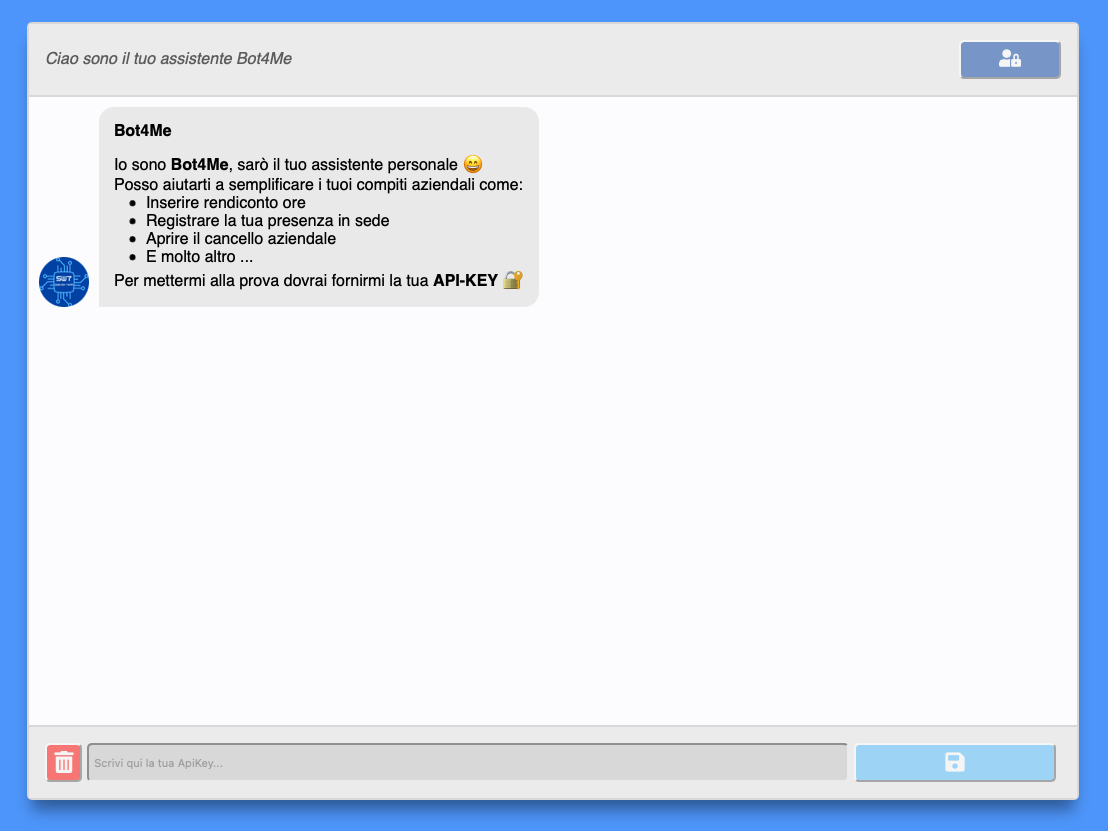
\includegraphics[width=0.9\textwidth, height=0.7\textheight, keepaspectratio]{images/schermata_avvio.png}
    \caption{Schermata Iniziale Bot4me}
\end{figure}

Inizialmente non si è loggati all'interno del sistema e per compiere qualsiasi tipo di operazione è necessario inserire un'\glossario{API-KEY} valida, ovvero che rispetti il formato suggerito da Imola Informatica, sarà poi compito del Server verificare se oltre che ad essere valida sia anche corretta per procedere con l'autenticazione. 

\subsection{Presentazione grafica e pulsanti}
\begin{itemize}
    \item Pulsante \textbf{Login / Logout:} in alto a destra il pulsante blu attualmente è solo per il login, dopo aver effettuato il login diventerà rosso per indicare il logout;
        \begin{figure}[H]
            \centering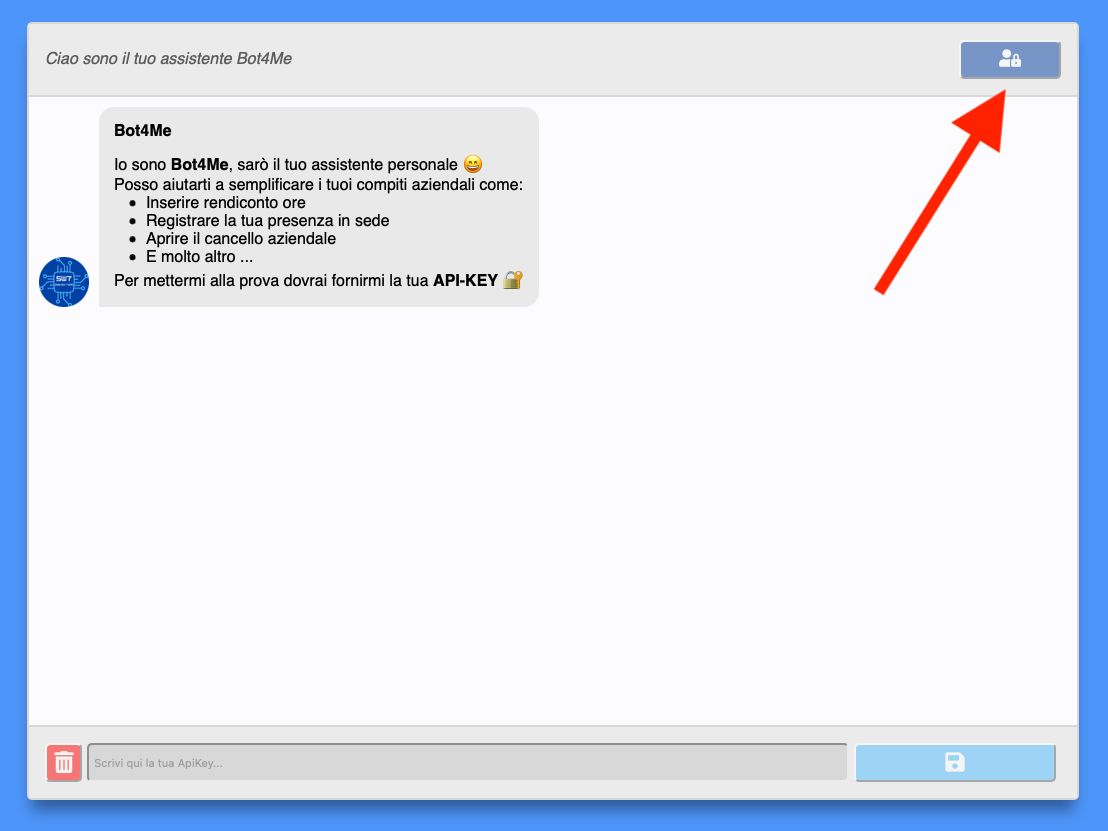
\includegraphics[width=0.8\textwidth, height=0.7\textheight, keepaspectratio]{images/schermata_pulsante_login.png}
            \caption{Pulsante - Login}
        \end{figure}
        \begin{figure}[H]
            \centering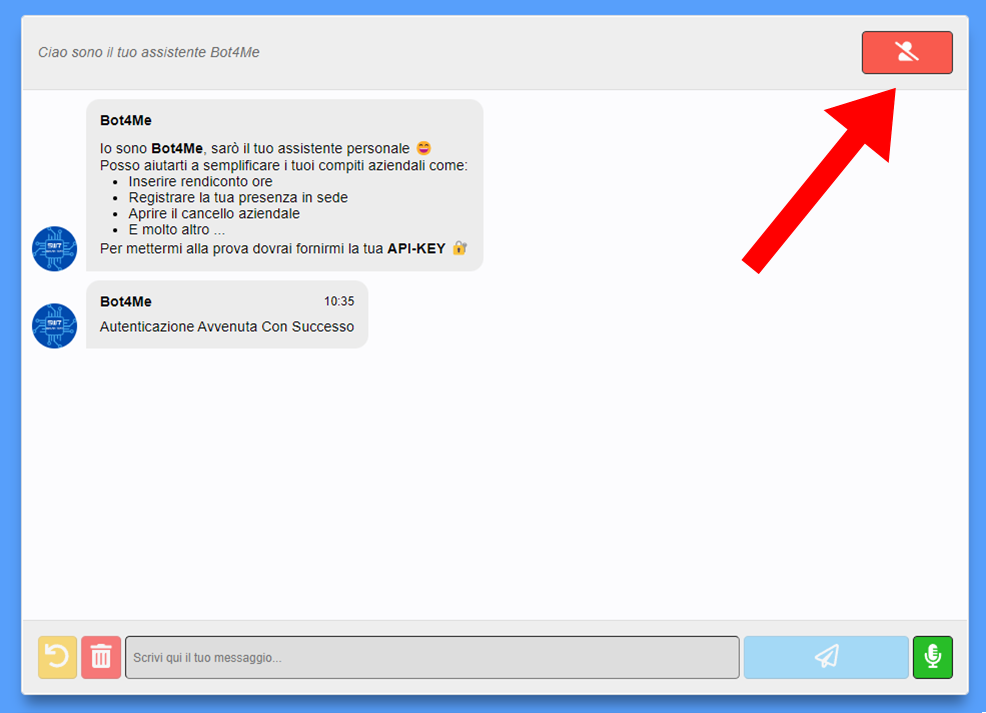
\includegraphics[width=0.8\textwidth, height=0.7\textheight, keepaspectratio]{images/schermata_pulsante_logout.png}
            \caption{Pulsante - Logout}
        \end{figure}
    \item Pulsante \textbf{Annulla:} in basso a sinistra il pulsante arancione serve per annullare la richiesta dell'operazione in corso, ritornando all'inizio. Non è possibile annullare un'operazione conclusa;
        \begin{figure}[H]
            \centering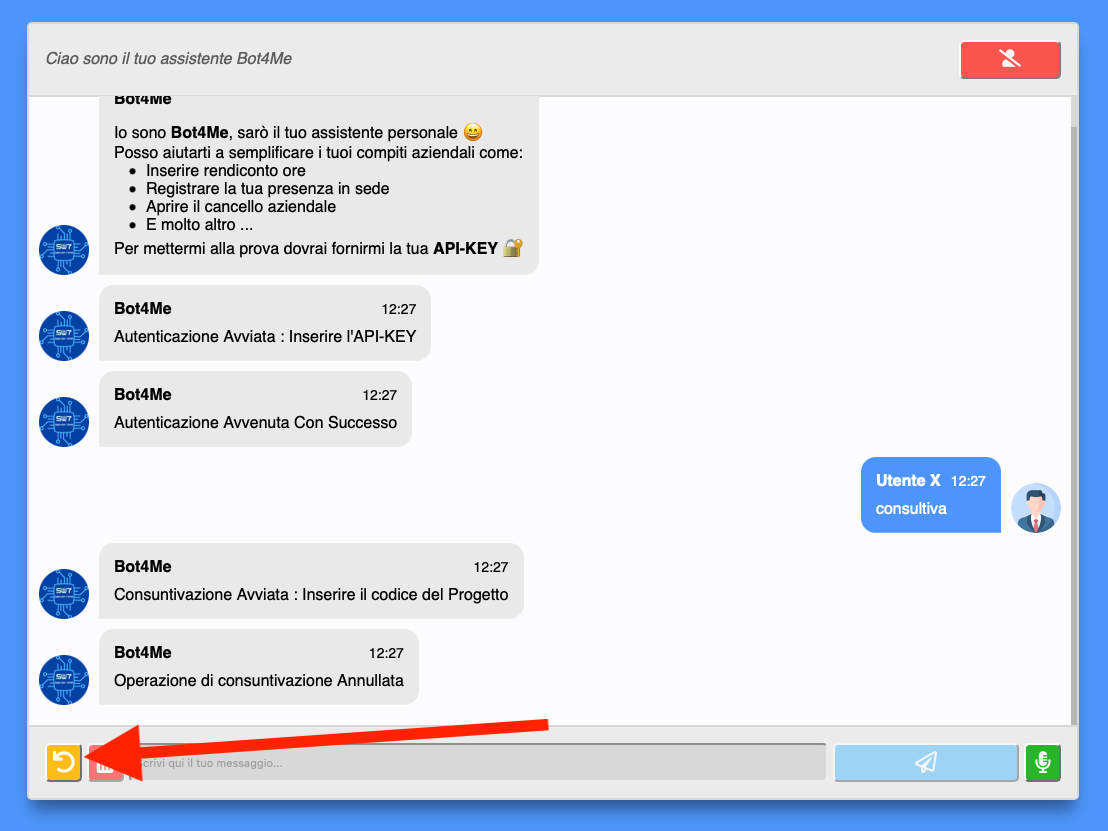
\includegraphics[width=0.8\textwidth, height=0.7\textheight, keepaspectratio]{images/schermata_pulsante_annulla.png}
            \caption{Pulsante - Annulla}
        \end{figure}
\newpage
    \item Pulsante \textbf{Elimina:} in basso a sinistra il pulsante rosso serve per cancellare ciò che si sta scrivendo, non è possibile premere il pulsante se la casella di testo è vuota;
        \begin{figure}[H]
            \centering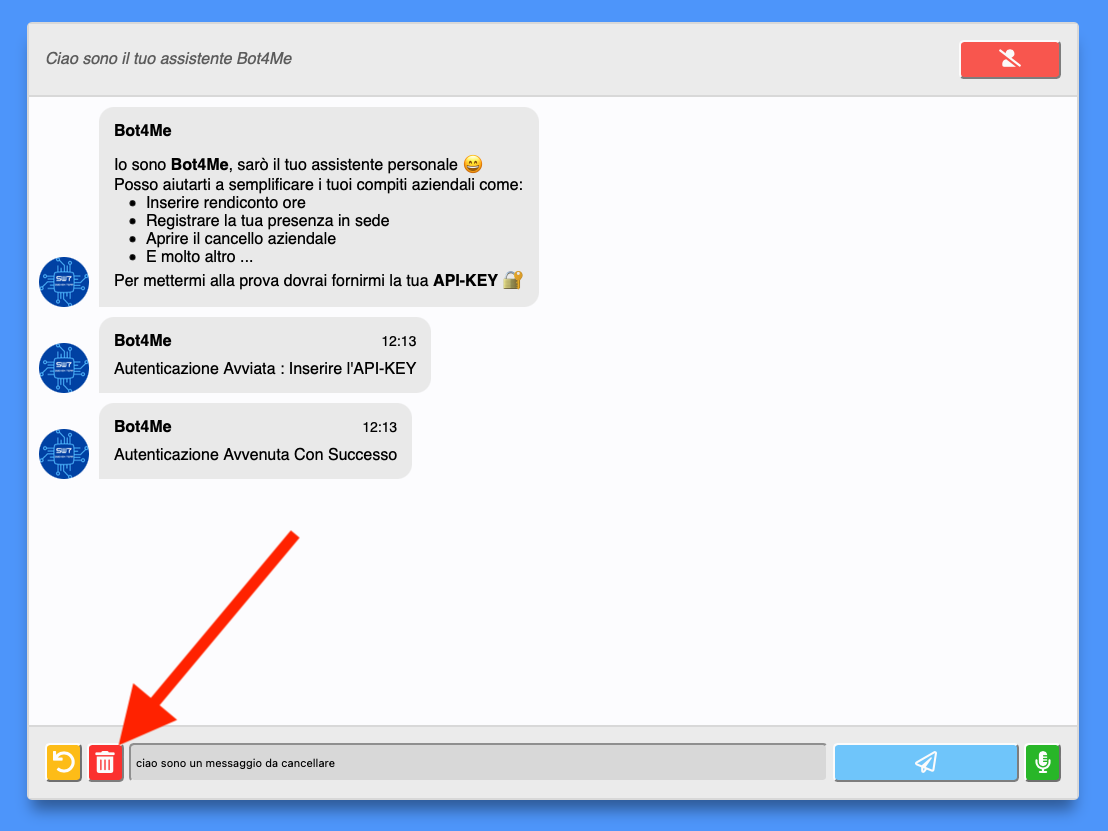
\includegraphics[width=0.8\textwidth, height=0.7\textheight, keepaspectratio]{images/schermata_pulsante_cancella.png}
            \caption{Pulsante - Elimina}
        \end{figure}
\newpage
    \item Pulsante \textbf{Invio:} in basso a destra il pulsante azzurro serve per inviare il messaggio scritto o alternativamente si può premere l'invio della tastiera;
        \begin{figure}[H]
            \centering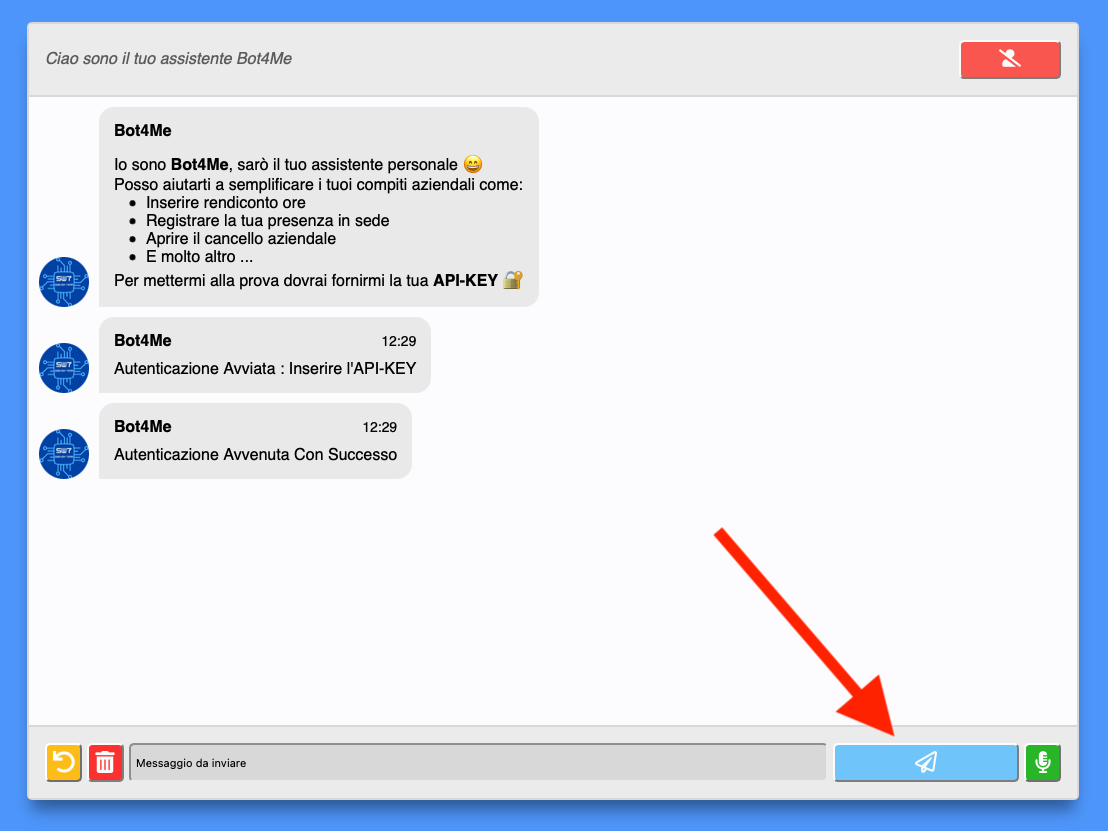
\includegraphics[width=0.8\textwidth, height=0.7\textheight, keepaspectratio]{images/schermata_pulsante_invio.png}
            \caption{Pulsante - Invio}
        \end{figure}
\newpage
    \item Pulsante \textbf{Vocale:} in basso a destra il pulsante verde serve per registrare vocalmente il messaggio che verrà automaticamente trascritto, con la possibilità di modificarlo manualmente nella casella di testo, e poi basterà cliccare sul pulsante azzurro o l'invio della tastiera; 
        \begin{figure}[H]
            \centering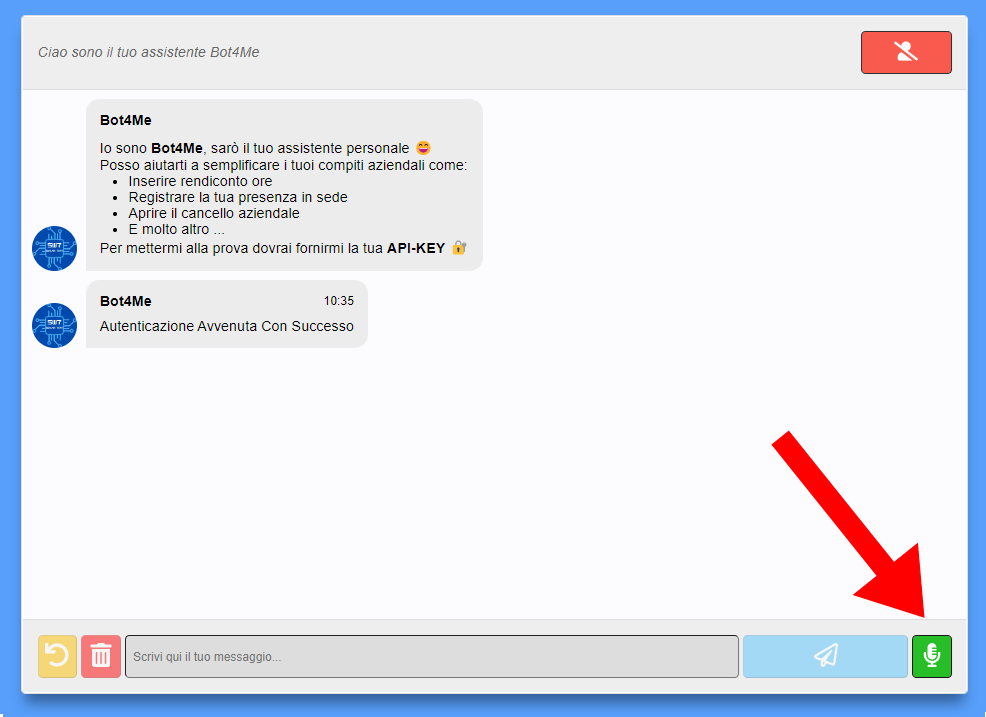
\includegraphics[width=0.8\textwidth, height=0.7\textheight, keepaspectratio]{images/schermata_pulsante_vocale.png}
            \caption{Pulsante - Vocale}
        \end{figure}

        \begin{figure}[H]
            \centering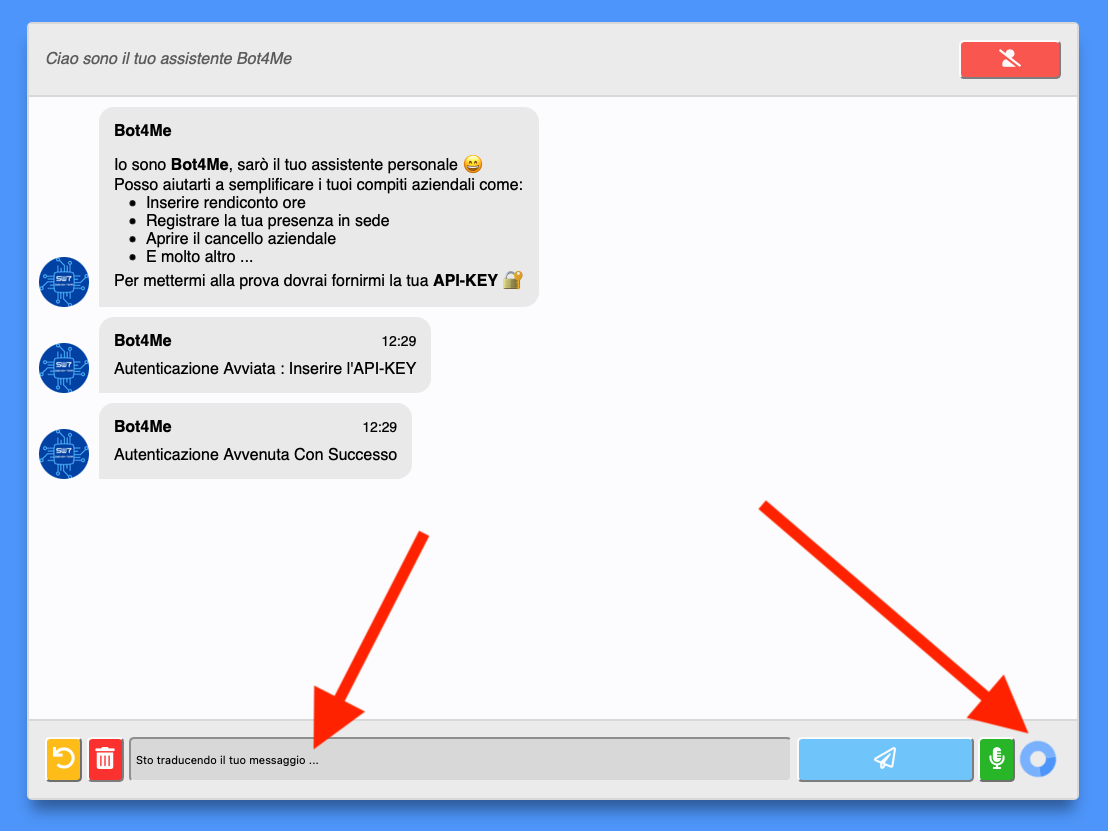
\includegraphics[width=0.8\textwidth, height=0.7\textheight, keepaspectratio]{images/schermata_pulsante_vocale_trascrizione.png}
            \caption{Trascrizione Messaggio Vocale}
        \end{figure}

\newpage
    \item Pulsante \textbf{Salva:} in basso a destra il pulsante azzurro con il simbolo di salvataggio, che prende il posto del pulsante d'invio e vocale, permette di salvare la propria \glossario{api-key} così da effettuare il processo di autenticazione.
    \begin{figure}[H]
        \centering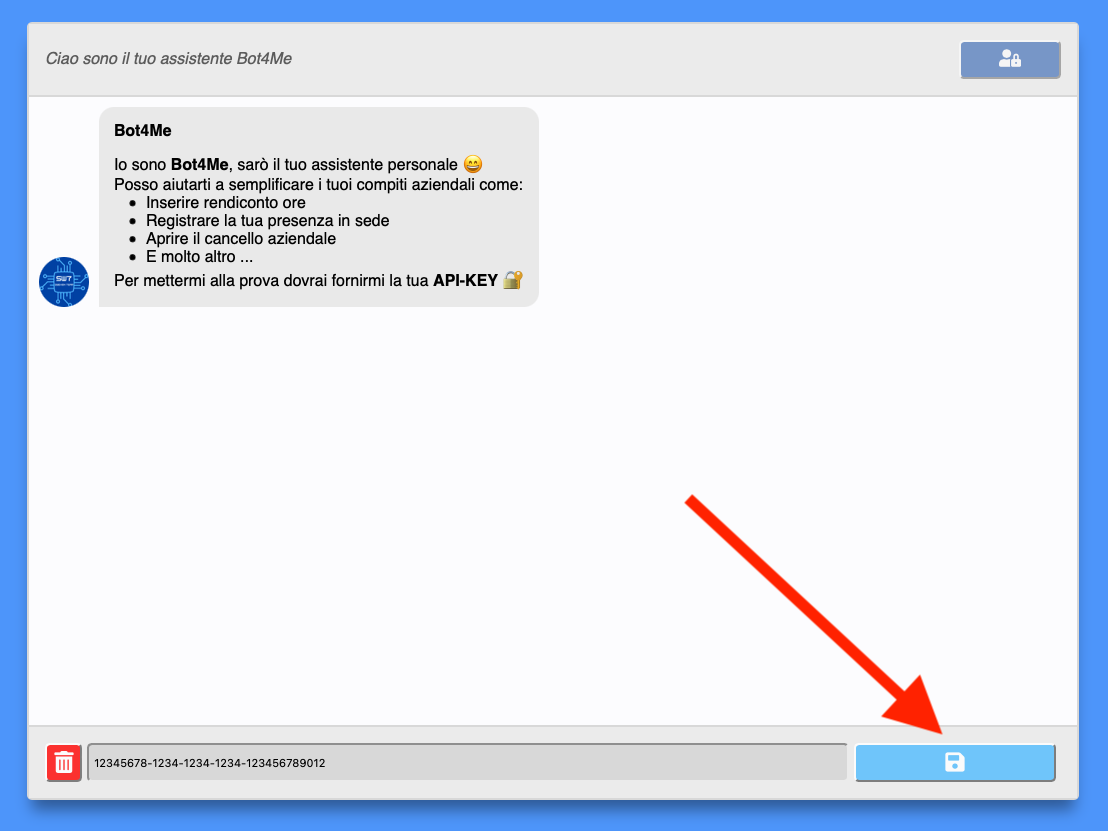
\includegraphics[width=0.8\textwidth, height=0.7\textheight, keepaspectratio]{images/schermata_pulsante_salva_API_KEY.png}
        \caption{Pulsante - Salva}
    \end{figure}
\end{itemize}

\newpage
\subsection{Autenticazione}
Per autenticarsi verrà chiesto di inserire la propria \glossario{API-KEY} di autenticazione all'avvio dell'applicazione. Se errata verrà comunicato che la richiesta è fallita, perchè l'\glossario{API-KEY} è risulta essere errata. Il chatbot verrà dunque ricaricato e si potrà effettuare un nuvoo tentativo; se risultasse essere corretta Bot4me comunica all'utente che l'autenticazione è avvenuta con successo e che può iniziare ad utilizzare i servizi che offre. 
Dopo l'autenticazione il pulsante in alto a destra diventerà di colore rosso con il simbolo di logout.
Se l'utente ricarica la pagina web, avviene un cambio di \glossario{UUID} e possono verificarsi due scenari: 
\begin{itemize}
    \item se l'utente ha effettuato il login in precedenza: la sua \glossario{API-KEY} risulta essere salvata all'interno del \glossario{Local-Storage} del browser, verrà dunque caricata all'interno della casella di testo e l'utilizzatore dell'applicazione potrà decidere se salvarla, tramite il bottone azzurro dotato dell'icona di salvataggio, effettuando così il login, oppure se modificarla e in seguito effettare l'autenticazione; 
    \item se l'utente non ha effettuato il login in precedenza: non sarà presente nessuna \glossario{API-KEY} all'interno del \glossario{Local-Storage} sarà dunque necessario inserirne una valida per procedere con la procedura di autenticazione. 
\end{itemize}

\subsubsection{Autenticazione - Inserimento \glossario{API-KEY}}
\begin{figure}[H]
    \centering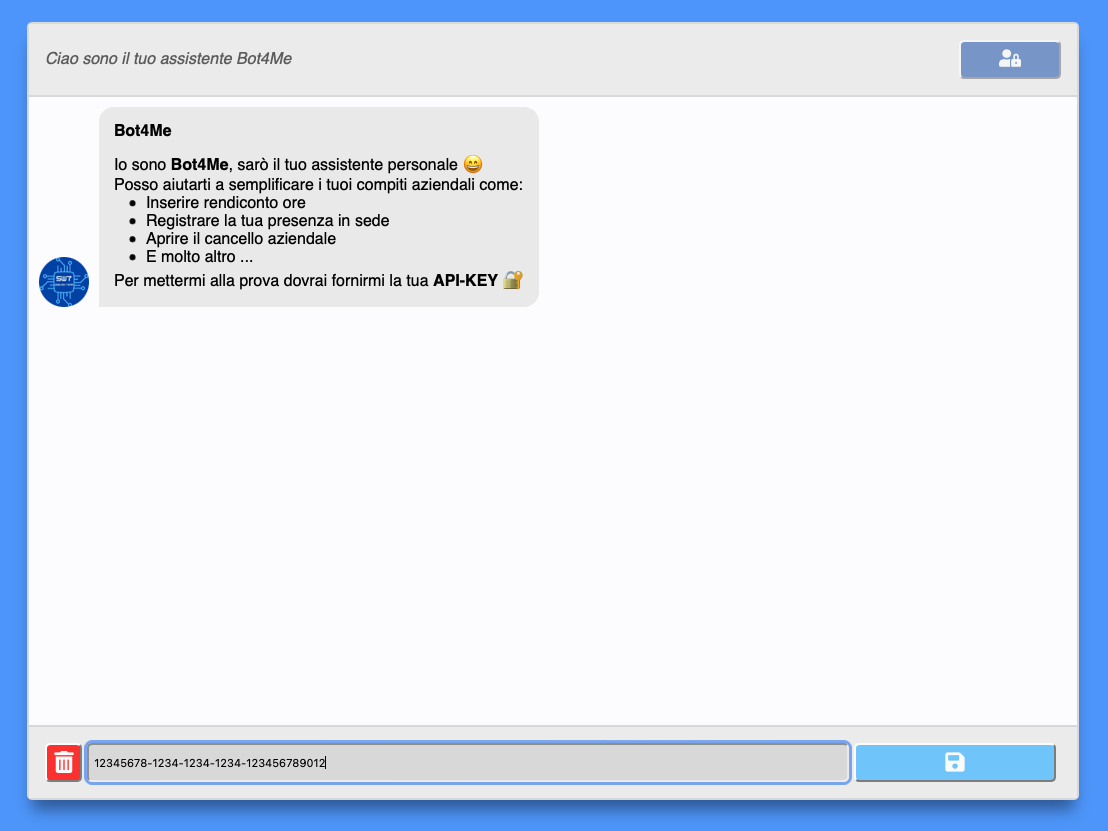
\includegraphics[width=0.9\textwidth, height=0.7\textheight, keepaspectratio]{images/schermata_autenticazione.png}
    \caption{Schermata Autenticazione Bot4me - Inserimento API-KEY}
\end{figure}

\newpage

\subsubsection{Autenticazione - Inserimento \glossario{API-KEY} Non Valida}
\begin{figure}[H]
    \centering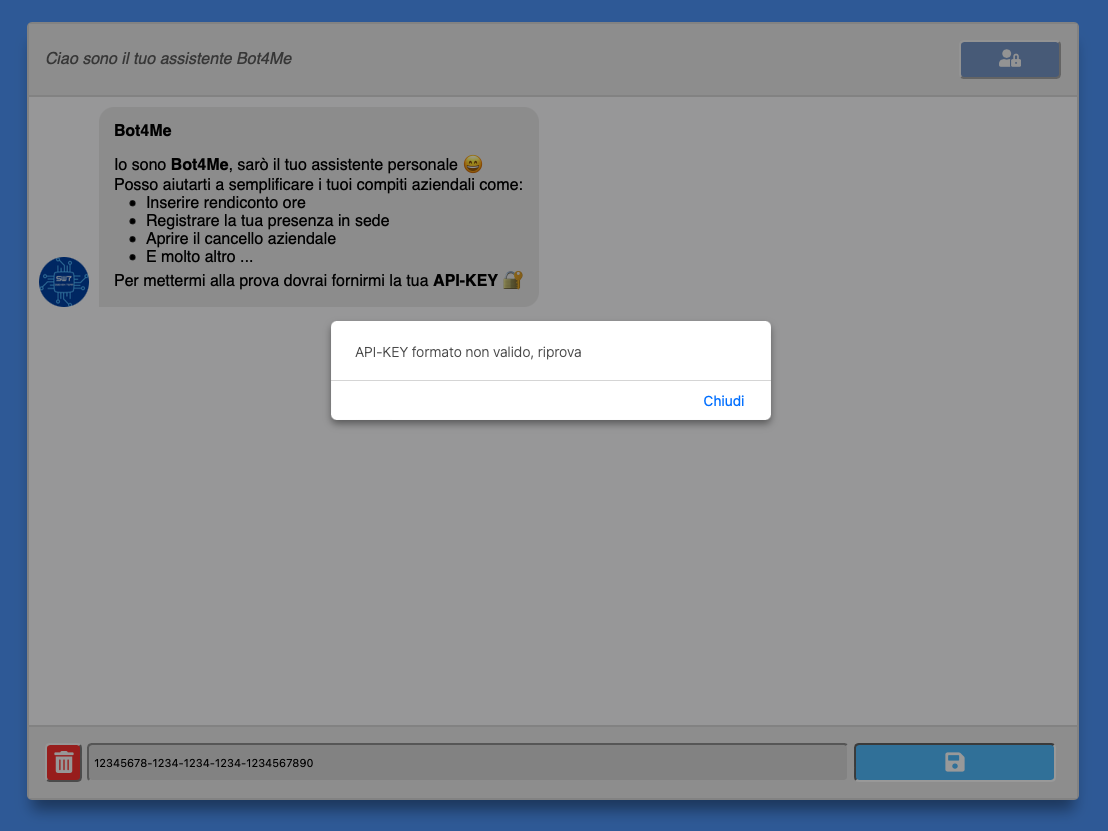
\includegraphics[width=0.9\textwidth, height=0.7\textheight, keepaspectratio]{images/schermata_autenticazione_apikey_non_valida.png}
    \caption{Schermata Autenticazione Bot4me - Inserimento API-KEY Non Valida}
\end{figure}

\subsubsection{Autenticazione Avvenuta con Successo - Inserimento \glossario{API-KEY} Valida e Corretta}
\begin{figure}[H]
    \centering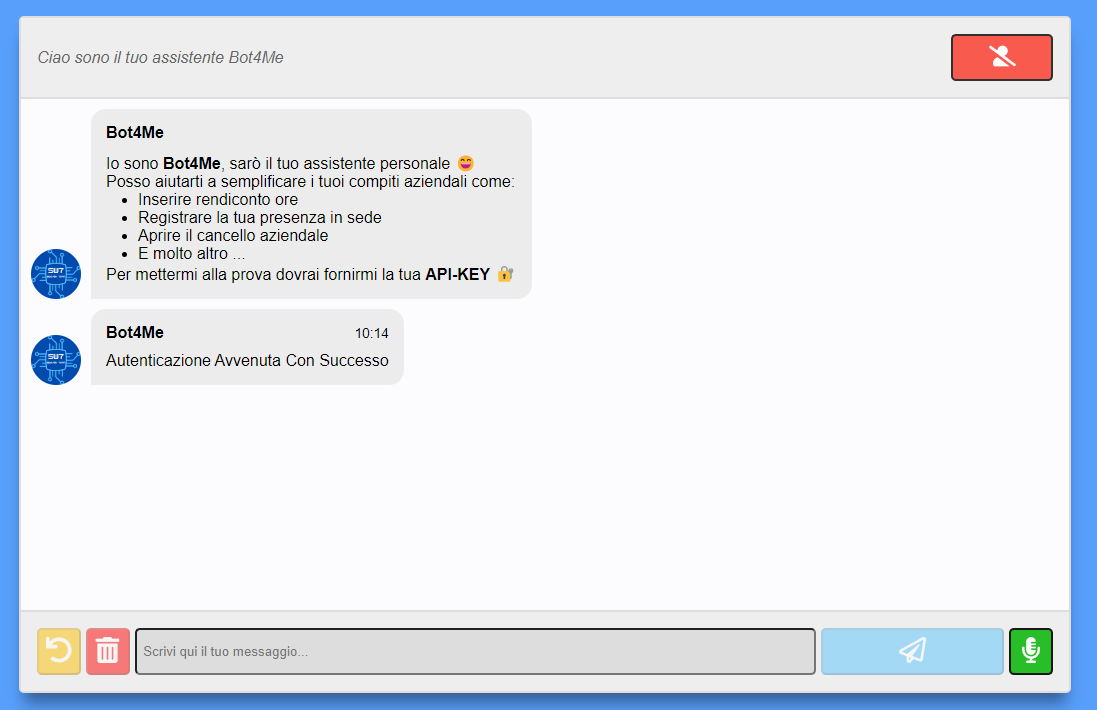
\includegraphics[width=0.9\textwidth, height=0.7\textheight, keepaspectratio]{images/schermata_autenticazione_successo.png}
    \caption{Schermata Autenticazione Avvenuta con Successo Bot4me - Inserimento API-KEY Valida e Corretta}
\end{figure}

\newpage